\documentclass{article}
\usepackage[utf8]{inputenc}
\usepackage{graphicx}
\begin{document}

\section{Abstract Classes}
\subsection{Definition}
An abstract class, in the context of Java, is a superclass that cannot be instantiated and is used to state or define general characteristics. An object cannot be formed from a Java abstract class; trying to instantiate an abstract class only produces a compiler error. The abstract class is declared using the keyword abstract.
Subclasses extended from an abstract class have all the abstract class's attributes, in addition to attributes specific to each subclass. The abstract class states the class characteristics and methods for implementation, thus defining a whole interface.
\subsection{Example}
We will illustrate the abstract class functionality by creating a small application that should act as a model, creating a Student database for a University. We will begin by defining an \textbf{abstract} Human class that reflects the idea of the Human characteristics that would be universal in the database.\\
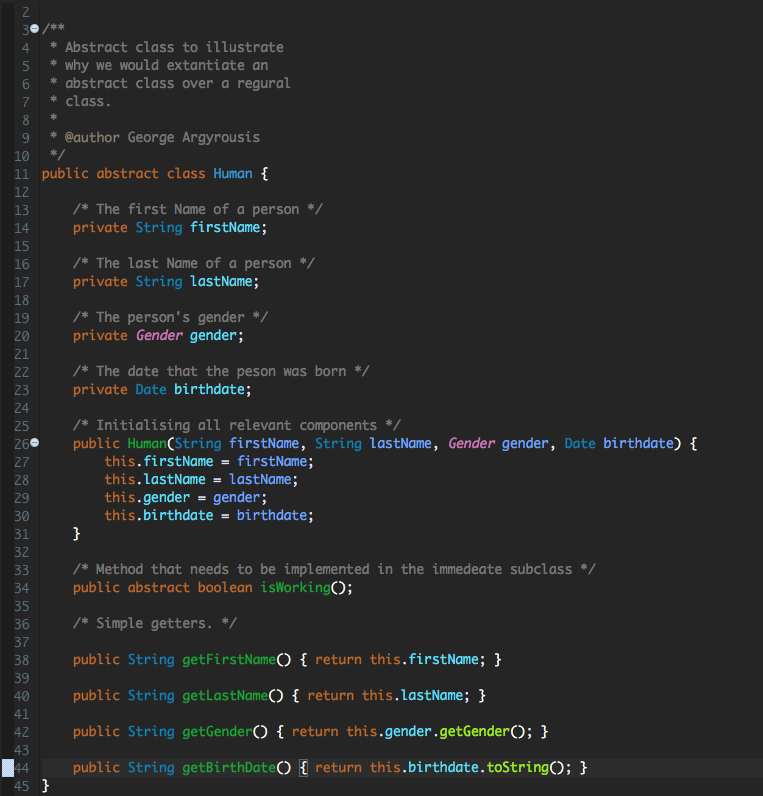
\includegraphics[scale=0.48]{images/Human.png}\\
We have defined attributes such as \textit{firstName}, \textit{lastName}, \textit{gender} and \textit{birthdate}. Representing common attributes among all humans. We have also defined one abstract method that will be implemented when the abstract class is extended by another regular class.\\
Of course we would not be able to create a \textbf{Human} object.\\
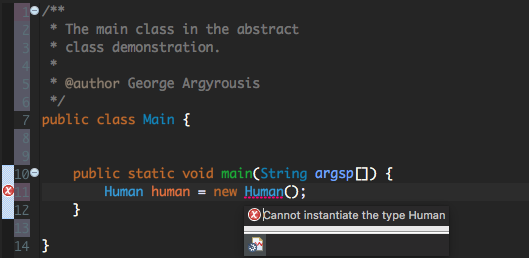
\includegraphics[scale=0.7]{images/Main_error.png}\\
Human is an abstract class that has defined general characteristics of the objects we would want in our database. We could possibly have multiple classes such as, \textbf{Professor}, \textbf{Student}, \textbf{Employee} that extend \textbf{Human}.\\
Thus inheriting all information provided by the abstract class itself. But we wouldn't want to have Human objects in the database as it is only reflecting the core idea.\\
We will proceed my making the \textbf{Student} object which extends Human.
A Student might have multiple other attributes but for this demonstration we will just add two ArrayLists and a StudentID.\\
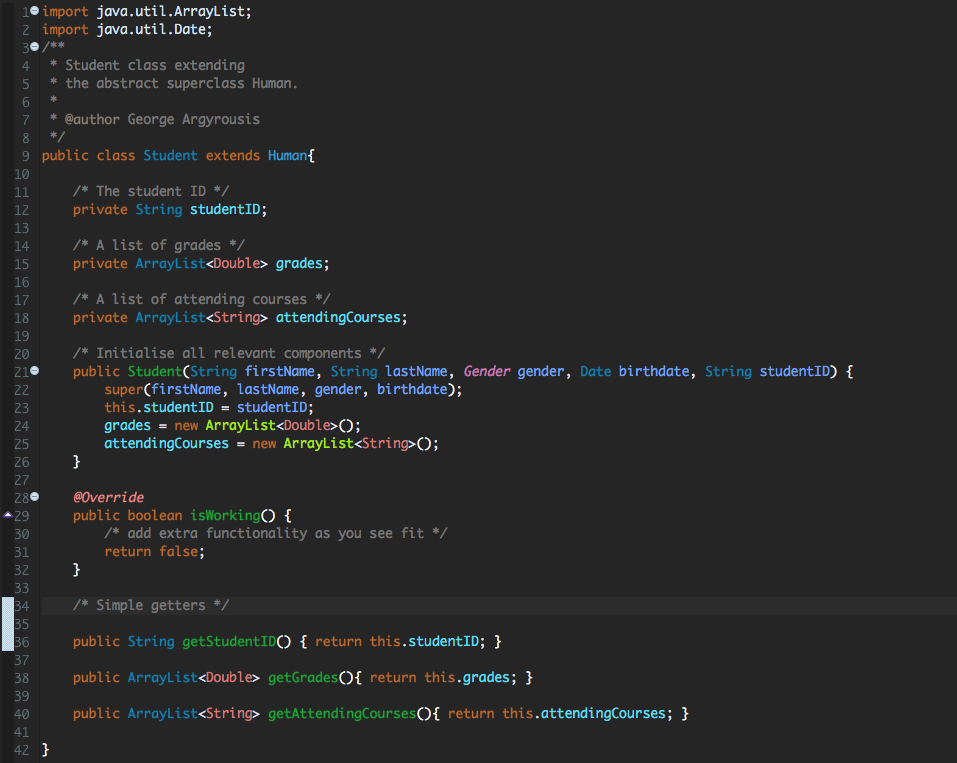
\includegraphics[scale=0.45]{images/Student_Step2.png}\\
Last but not least, we initialize the object and print it's attributes in the
command line.\\
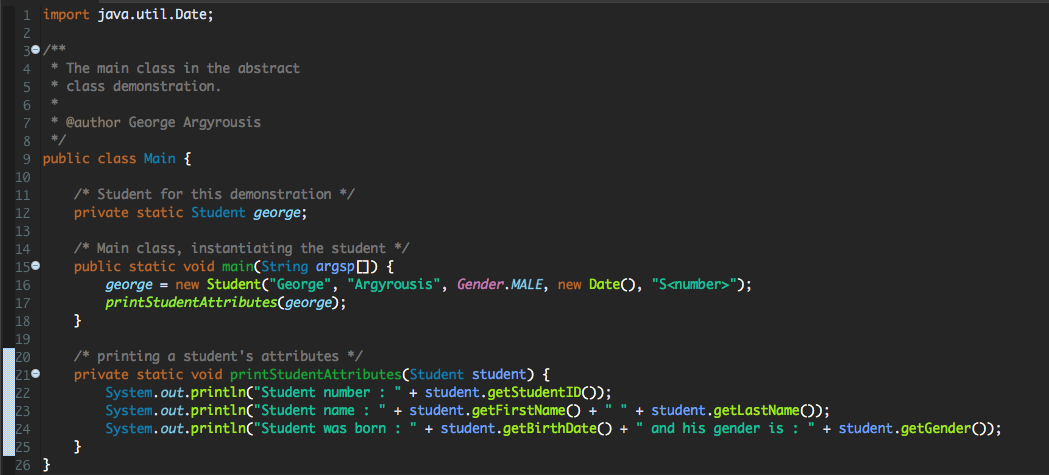
\includegraphics[scale=0.40]{images/Main_without_error.png}\\
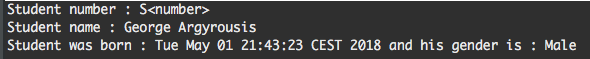
\includegraphics[scale=0.71]{images/output.png}\\
\end{document}
